\documentclass[11pt,a4paper]{article}

\usepackage[margin=1in]{geometry}
\usepackage{amsmath,amssymb,amsthm}
\usepackage{booktabs}
\usepackage{enumitem}
\usepackage{graphicx}
\usepackage{hyperref}
\usepackage{parskip}

\hypersetup{colorlinks=true, linkcolor=blue, urlcolor=blue}

\newtheorem{theorem}{Theorem}
\newtheorem{claim}{Claim}
\newtheorem{remark}[theorem]{Remark}

\newcommand{\keyidea}[1]{\medskip\noindent\textbf{Key idea.}\ #1\medskip}
\newcommand{\econ}[1]{\medskip\noindent\textbf{Economics.}\ #1\medskip}

\title{\textbf{Fundamental Theorem of Linear Programming}\\[0.2em]
\large Math Camp 2026 --- Teaching Notes}
\author{}
\date{}

\begin{document}
\maketitle

\begin{center}
\small
\textit{On a nonempty polyhedron, a bounded linear objective attains its optimum.\\
The geometry: a sliding hyperplane must touch a flat face.}
\end{center}

\tableofcontents
\newpage

%==============================================================================
\section{Statement}
%==============================================================================

Linear programs ask for the best value of a linear function over a polyhedron.
The fundamental theorem says that if the value is finite, an optimizer actually exists.

\begin{theorem}[Fundamental theorem of linear programming]
Let $P=\{\mathbf{x}\in\mathbb{R}^n: A\mathbf{x}\le\mathbf{b}\}$ be a nonempty polyhedron and let
$f(\mathbf{x})=\mathbf{c}^{\mathsf T}\mathbf{x}$.
If $f$ is bounded above on $P$, i.e.\ $\sup_{\mathbf{x}\in P}\mathbf{c}^{\mathsf T}\mathbf{x}<\infty$,
then $f$ attains its maximum on $P$: there exists $\mathbf{x}^*\in P$ with
$\mathbf{c}^{\mathsf T}\mathbf{x}^*=\sup_{\mathbf{x}\in P}\mathbf{c}^{\mathsf T}\mathbf{x}$.
\end{theorem}

The same statement holds for a minimum when $f$ is bounded below (apply the theorem to $-f$).
We focus on maximisation below.

\begin{remark}[This fails for general closed sets]
Closedness and a finite supremum are not enough.
Take $P=\{(x,y)\in\mathbb{R}^2: y\ge e^x\}$ and $f(x,y)=-y$.
Then $f\le 0$ on $P$, so $\sup f=0$, but no point in $P$ has $f=0$.
The set approaches the horizontal line $y=0$ asymptotically; its boundary is curved.
Polyhedra are different: finitely many flat faces, no such asymptotic gaps.
\end{remark}

\econ{In LP applications (profit maximisation, cost minimisation), ``the optimum value is $M$'' is only
useful if some feasible plan actually achieves $M$.
This theorem guarantees that when the problem is well posed (nonempty feasible set, finite optimum),
an optimal solution exists.}

The proof is geometric: slide a family of parallel hyperplanes until the last one still touches $P$.

%==============================================================================
\section{Geometric proof: the sliding hyperplane}
%==============================================================================

Fix $\mathbf{c}\neq\mathbf{0}$ and write $M=\sup_{\mathbf{x}\in P}\mathbf{c}^{\mathsf T}\mathbf{x}$.
Consider the parallel hyperplanes
\[
  H_t = \{\mathbf{x}\in\mathbb{R}^n : \mathbf{c}^{\mathsf T}\mathbf{x}=t\},
  \qquad t\in\mathbb{R}.
\]
As $t$ increases, $H_t$ moves in the direction of $\mathbf{c}$.
Since $M$ is finite, $H_t$ misses $P$ for all $t>M$, and $H_t$ meets $P$ for some $t\le M$.
The claim is that the highest touching hyperplane is $H_M$ itself.

\keyidea{Project $P$ onto the line spanned by $\mathbf{c}$.
For a polyhedron, this projection is a \textbf{closed} interval with right endpoint $M$;
hence $M$ is attained.}

\begin{claim}[Closed projection]
Let $S=\{\mathbf{c}^{\mathsf T}\mathbf{x}:\mathbf{x}\in P\}\subset\mathbb{R}$.
Then $S$ is a closed interval of the form $(-\infty,M]$ or $[a,M]$ for some $a\le M$.
In particular, $M\in S$.
\end{claim}

\begin{proof}[Proof sketch]
A polyhedron is an intersection of finitely many halfspaces, so $P$ is closed and convex.
The linear map $\mathbf{x}\mapsto\mathbf{c}^{\mathsf T}\mathbf{x}$ sends $P$ to a closed convex subset of
$\mathbb{R}$, hence an interval.
Since $M$ is the supremum of $S$, the interval is bounded above with right endpoint $M$.
Closedness of the image forces $M\in S$: otherwise $S\subset(-\infty,M)$, contradicting that $M$ is the
\emph{least} upper bound.
Any $\mathbf{x}^*\in P$ with $\mathbf{c}^{\mathsf T}\mathbf{x}^*=M$ is optimal.
\end{proof}

\textbf{Why polyhedra are special (2D picture).}
Rotate coordinates so $\mathbf{c}=(1,0)^{\mathsf T}$; then $f(\mathbf{x})=x_1$ and $H_t$ is the vertical line
$x_1=t$.
The projection $S$ is the set of first coordinates of points in $P$.
A polygon cannot approach $x_1=M$ asymptotically: boundary edges are straight segments.
A line either crosses $x_1=M$ (impossible if $M$ is the supremum), lies on $x_1=M$ (a vertical face, so $M$
is attained), or turns away earlier (the rightmost point is then a vertex).
So the right boundary is built from finitely many closed edges and vertices, and $P\cap H_M\neq\emptyset$.

\begin{center}
  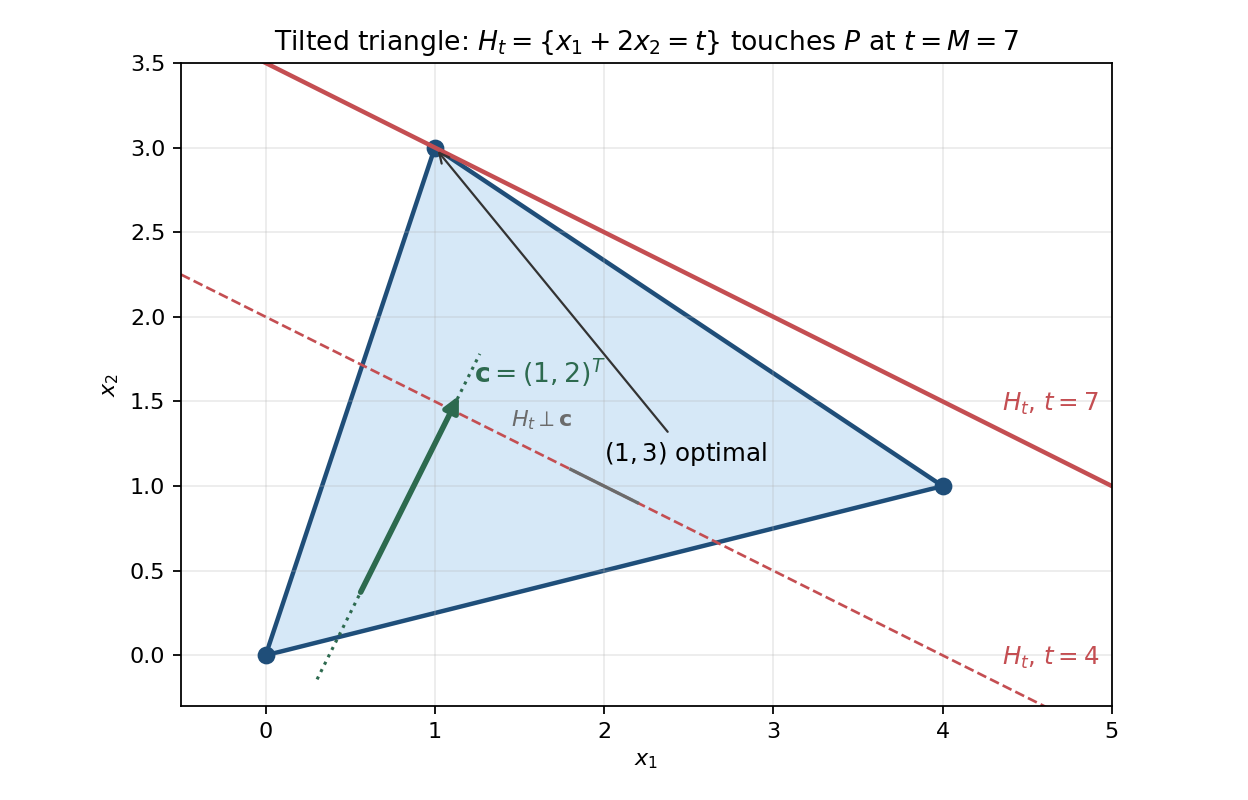
\includegraphics[width=0.78\textwidth]{figures/sliding_hyperplane.png}
\end{center}

\textbf{Example (tilted triangle, tilted objective).}
Let $P$ be the triangle with vertices $(0,0)$, $(4,1)$, and $(1,3)$, and take $\mathbf{c}=(1,2)^{\mathsf T}$,
so $f(\mathbf{x})=x_1+2x_2$.
The hyperplanes $H_t=\{\mathbf{x}: x_1+2x_2=t\}$ are \emph{tilted} lines (not vertical).
Evaluating at the vertices gives $f=0$, $6$, and $7$, so $M=7$ and the maximum is attained at
$(1,3)$.
The highest hyperplane $H_7$ touches $P$ at that vertex; for $t>7$ the line misses the triangle entirely.

\begin{remark}[Unbounded polyhedra]
$P$ may be unbounded (e.g.\ a wedge opening to the left).
If $f$ is still bounded above, no recession direction of $P$ can increase $\mathbf{c}^{\mathsf T}\mathbf{x}$.
The right ``cap'' is still cut out by finitely many bounding hyperplanes, so the same closed-projection
argument applies.
\end{remark}

\keyidea{Suprema are attained on polyhedra because boundaries are \textbf{flat}, not curved.
The sliding hyperplane stops on a face; that face contains an optimizer.}

\end{document}
